\section{رویکرد و راه‌حل}

رویکر و روش‌شناسی‌ای که این مقاله در مورد آن صحبت می‌کند توضیح‌پذیری در
سیستم‌های نرم‌افزاری و حتی مدل‌های هوش مصنوعی است تا بتواند ضعف عدم شفافیت
سیستم‌ها را رفع کند.در این مقاله، بنا به ضرورت توضیح‌پذیری سیستم های نرم افزاری،
به صورت روشی مناسب، سعی بر آن دارد تا توضیح‌پذیری را بیان کند و به صورت شفاف به
عنوان یک نیازمندی غیرعملیاتی ابعاد مختلف آن را روشن سازد. همچنین در مورد رابطه
بین جنبه‌های کیفی نیز صحبت می‌کند.

\subsection{توضیح‌پذیری چیست؟}

توضیح‌پذیری یک روش مفید است تا از نگرانی‌های اخلاقی نرم‌افزار‌ها و مدل‌ها بکاهد.
به معنای قابلیت شرح نرم‌افزار و سیستم است. وقتی یک سیستم یا مدل هوش مصنوعی
توضیح‌پذیر است، به این معناست که عملکرد و تصمیمات آن قابل تفسیر و توجیه است. به
عبارت دیگر، می‌توان به راحتی فهمید که یک سیستم به چه شکلی کار می‌کند و چگونه به
تصمیمات خود رسیده است. توضیح‌پذیری یک ویژگی بسیار مهم در سیستم‌های نرم‌افزاری
است که موجب افزایش اعتماد به آن می‌شود و ارزش‌های اخلاقی و قانونی را در رابطه با
سیستم تعریف خواهد کرد. امروزه به مسئله توضیح‌پذیری سیستم‌ها بسیار اهمیت داده
می‌شود و یکی از مهم‌ترین نیازمندی‌های غیرعملیاتی \footnote{\lr{Non-functional}}
محسوب می‌شود. در حالتی که به کاربران این اجازه را می‌دهد که خودشان بتوانند
انتخاب کنند که از این سیستم استفاده کنند یا از آن دوری کنند چرا که بر روی رابطه
قابلیت اعتماد و اتکای سیستم بسیار تاثیرگذار می‌باشد.

نکته: با توجه به قدرت هوش مصنوعی در تمام حوزه‌های زندگی بشر، توضیح‌پذیری به
عنوان یکی از مهم‌ترین پایه‌های اعتماد در نیازمندی‌های نرم‌افزار می‌باشد.

\subsection{چالش‌های توضیح‌پذیری}

دلایل زیر نشان‌دهنده آن است که جمع‌آوری و استخراج داده، مذاکره و اعتبارسنجی در
فرایند توضیح‌پذیری با چالش‌هایی رو به رو می‌باشد:

\subsubsection{پیچیدگی سیستم‌ها}

در سیستم‌هایی که مبنی بر هوش مصنوعی و فرایند یادگیری ماشین هستند با وجود
الگوریتم‌های مختلف که وظیفه تصمیم‌گیری را در سیستم دارند، سطح پیچیدگی بسیار بالا
می‌باشد. درک و توضیح این سیستم‌ها با فرایند‌هایشان برای کاربران مختلف به مفهوم
ساده، بسیار سخت و غیرقابل درک می‌باشد.

\subsubsection{طبعیت \lr{Black box}}

از نظر کاربران، بسیاری از الگوریتم‌ها به شکل جادویی عمل می‌کنند، بدان معنا که
فرایند‌های داخلی این الگوریتم‌ها کاملا به صورت مات می‌باشد و توسط انسان بدون
دانش قبلی به راحتی قابل درک نیست.

\subsubsection{وابستگی توضیح‌پذیری به ذهنیت افراد \lr{Subjectivity of
Explanation}}

زمینه‌گرایی توضیح به معنای نسبی بودن یا وابستگی توضیحات به نگرش و دیدگاه فردی
است. در حالت کلی تفسیر هر چیزی توسط ذینفعان می‌تواند کاملا متفاوت از نظر معنا و
دیدگاه باشد. مذاکره برای به اجماع رسیدن در سطح و نوع توضیح مورد نیاز می‌تواند
چالش برانگیز باشد، به ویژه زمانی که با دیدگاها و علایق گوناگون سروکار داریم.

\subsubsection*{عدم درک مشترک \footnote{\lr{Lack of shared understanding}}}

یکی دیگر از دشواری‌ها، ارتباطات مناسب در مهندسی نیازمندی است. ذینفعان بیرونی و
تیم توسعه ممکن است ناخواسته از یکسری کلمات متفاوت با مفهوم یکسان استفاده کنند که
در نهایت باعث ایجاد سوء‌تفاهم و نقص فهم مشترک بین افراد شود که در نهایت چالشی
برای ارتباط با یکدیگر ایجاد می‌کند. لازمه کارآمدی ارتباطات درک مشترک از مفاهیم
می‌باشد که ریسک دوباره‌کاری و نارضایتی ذینفعان را کاهش می‌دهد.

\subsubsection*{رویکرد درک مشترک بین افراد}

مهندسان نرم‌افزار می‌توانند مجموعه‌ای از فرآورده‌ها را ایجاد کنند که باعث ایجاد
درک و فهم مشترک در پروژه‌های نرم‌افزاری می‌شود و بار‌ها قابل استفاده مجدد و
اصلاح خواهند بود تا فرآورده‌ها، محصولی از مذاکره با زبانی مشترک بین افراد باشد.

\subsubsection*{فرآورده‌ها}

فرآورده‌ها هر گونه اسناد متنی و اشکال گرافیکی هستند که به دور از کد‌ها و
محصولاتی نرم‌افزاری، ابزاری برای مذاکره بین تمام افراد‌ حاضر (چه ذینفعان چه
مهندسان مختلف) می‌باشند. محتوای فرآورده‌ها معمولا اشکال، متن‌ها، مدل‌های بصری،
فهرست‌ها، چارت‌ها ، چهارچوب‌ها و مدل‌های کیفیت می‌باشد. این فرآورده‌ها در
شکل‌دهی ساختار پروژه بسیار کارآمد هستند به گونه‌ای که در فرایند‌های مهندسی
نیازمندی از قبیل، مدل‌های مفهومی \footnote{\lr{Conceptual models}} کاتالوگ دانش
\footnote{\lr{Knowledge catelogues}} و مدل‌های مرجع \footnote{\lr{Reference
models}} کاربرد متعددی دارند.

\subsubsection{رابطه الاکلنگی بین توضیح‌پذیری و عملکرد}

با افزایش توضیح‌پذیری ممکن است کارایی سیستم کاهش یابد. در نتیجه لازم است بین این
نیازمندی با سایر نیازمندی‌ها تعادل ایجاد شود. راهکار ایجاد تعادل می‌تواند موارد
زیر باشد:

% \subsubsection{تریدآف همراه با تاثیرگذاری روی عملکرد یا \lr{Trade-off with
% Performance}}

% گاهی افزایش توضیح‌پذیری در یک سیستم می‌تواند به قیمت عملکرد و کارایی تمام شود.
% یک مهندس نیازمندی باید بتواند بین توضیح‌پذیری با سایر الزامات سیستم \lr{System
% requirements} تعادل  ایجاد کند. برای درک این چالش مثال زیر را مطالعه کنید:

% تصور کنید یک شرکت در حال توسعه سیستم توصیه‌گرا برای اپلیکیشن تجاری خود می‌باشد.
% این سیستم الگوریتم‌های پیچیده \lr{ML} را برای تحلیل رفتار‌ها و ترجیحات
% \footnote{\lr{Preferences}} کاربران استفاده می‌کند تا بتواند محصولات مشابه
% علاقه‌مندی آنها را به نحوی معرفی کند که کاربران انتظار داشتند. یکی از
% نیازمندی‌های \lr{NFR} این سیستم، ارائه توضیحات برای هر کدام از نتایج محصولات
% توصیه شده می‌باشد تا بتواند موجب اعتماد و رضایت کاربران شود. در این صورت گنجاندن
% توضیحات به همراه جزئیات چرایی انتخاب این مورد (محصول) به عنوان مورد مرتبط برای
% این سیستم تاثیر به سزایی در عملکرد آن خواهد داشت. این عمل باعث تاخیری در تولید
% این موارد برای کاربران می‌شود که از نظر تجربه کاربری \footnote{\lr{User
% experience}} یک ضعف محسوب می‌شود به ویژه زمانی که کاربران انتظار دارند که تمام
% تقاضا‌هایشان از سیستم در کمتر از پنج ثانیه پاسخ داده شود.

% احتمالاً برای این مثال راهکار‌های زیر در نظر گرفته می‌شود تا ضمن توضیح‌پذیری
% سیستم، عملکرد سیستم نیز مانند سابق با سرعت بالا حفظ شود:

\begin{enumerate}
    \item کاهش پیچیدگی توضیحات: به جای آنکه توضیحات کاملی در مورد عملکرد
    الگوریتم‌های هوش مصنوعی به ازای هر مورد فراهم شود، سیستم می‌تواند بسیار ساده
    با ارائه خلاصه‌ای مفید، فاکتور‌های مهم و اساسی دلیل انتخاب موارد به عنوان
    توصیه کاربر را مشخص کند.
    \item استفاده از متد‌های فنی در مهندسی نرم‌افزار مانند فرایند‌های کش کردن
    انتخاب‌های کاربر (براساس کلیک‌های مختلف روی محصولات یا مدت زمانی که روی
    محصول مورد نظر کاربر مطالعه داشته) محاسبات از پیش تعیین شده‌ای در مورد چرایی
    انتخاب محصول به عنوان توصیه را مشخص کند.
\end{enumerate}

انتخاب استراتژی مناسب برای حفظ توضیح‌پذیری به همراه سرعت و کارایی بالا در عملکرد
سیستم توصیه‌گرا، یک تریدآفی است که وظیفه آن بر عهده تیم توسعه، طراح و معماری
نرم‌افزار می‌باشد.

\subsubsection{سیستم‌های پویا و در حال تکامل}

یکی از چالش‌های مهم توضیح‌پذیری، سیستم‌هایی است که در طول زمان دچار تغییرات کلی
به ویژه در نیازمندی‌ها می‌شوند. اینکه توضیحات متناسب با تغییر سیستم‌ها به روز
شود چالشی مهم است.

\subsubsection{اعتبارسنجی و اعتماد}

اعتبار بخشیدن به توضیحات ارائه شده توسط یک سیستم می تواند دشوار باشد، به ویژه
زمانی که آنها شامل فرآیندها یا داده های پیچیده باشند. ایجاد اعتماد در این
توضیحات مستلزم روش‌های اعتبارسنجی قوی و شفافیت در فرآیند تولید توضیح است.

همچنین اشاره می‌کند که مهندسی نیازمندی فرایند ساده برای شناسایی و مشخص کردن
نیازمندی‌ها نیست، بلکه فرایندی جهت حمایت از ارتباطات کارآمد این نیازمندی‌ها بین
ذینفعان مختلف می‌باشد.

مهم ترین مشکل در زمینه توضیح‌پذیری، کمبود دانش ساخت‌یافته می‌باشد. اگر چنین
دانشی به وجود بیاید به مهندسی نرم افزار کمک می‌کند فاکتورهایی را طی روند
پیاده‌سازی سیستم‌های توضیح‌پذیر در نظر بگیرد تا به درک مشترک کمک کند. 

\section{سابقه دانشی و مدل پیشنهادی}

برای اجماع فهم مشترک بر مسائل مختلف این حوزه از مهندسی نرم‌افزار، خواننده نیاز
دارد که با مفاهیم زیر به صورت کلی آشنا باشد تا بتواند:

\begin{enumerate}
    \item از دانشی فراتر از زمینه‌های خود استفاده کنند و از این دانش برای رفع
    نیاز‌های یک پروژه خاص (جاری یا جدید) استفاده کنند.
    \item دستیابی به درکی مشترک که منجر به ارتباطات بهتر و تعریف نیازمندی‌های
    سیستم به شکل «درست» می‌شود.
\end{enumerate}

در این مقاله توضیح‌پذیری به صورت چهار فرآورده \footnote{\lr{Artifact}} به صورت
روشمند و منطبق با چرخه عمر نرم‌افزار تبیین شده است. این چهار سطح عبارتند از: 

\subsection{تعاریف یا \lr{Definitions}}

تعاریف در مهندسی نرم‌افزار و مهندسی نیازمندی، راهنمایی تقریبی برای مهندسان
نرم‌افزار در مورد دامنه، عناصر و هر چیز دیگری را ارائه می‌دهند. به این صورت که
یکی از مهم‌ترین مراحل تسهیل ارتباطات برای یک موضوع یا یک مفهوم می‌باشند. وقتی در
مورد تعریف جنبه‌های کیفی \footnote{\lr{Quality aspects}} صحبت می‌شود در حقیقت
منظور همان راهنمایی‌ها برای مهندسان نرم‌افزار است که به آنها در فهمیدن روند
مهندسی نیازمندی به خصوص تضمین کیفیت \footnote{\lr{Quality assurance}} کمک
می‌کند. عدم اجماع حاضرین بر سر مفاهیم و تعاریف می‌تواند سبب ایجاد نتیجه نامناسبی
در مشخصات و یکپارچگی نیازمندی‌های غلط شود. برای مثال وقتی در جلسات در مورد
\lr{Usability} صبحت می‌شود، برخی از افراد توسعه دهنده منظور را در رابطه با
استفاده و بهره‌وری بلند مدت \footnote{\lr{Long-term efficiency}} می‌دانند و برخی
از افراد منظور را در استفاده آسان محصول \footnote{\lr{Ease of Use (EoU)}}
می‌دانند.

\subsection{مدل‌ها یا \lr{Models}}

یک مدل در بالاترین سطح تجرید در مورد کارایی سیستم تمرکز دارد که بتواند تمام
جنبه‌های سیستم را به سادگی و به دور از جزئیات نمایش دهد. هیچ وقت یک مدل به
تنهایی، تمام سیستم را تشریح نمی‌کند. مدل‌ها در طیف گسترده‌ای از جنبه‌های مختلف
یک سیستم استفاده می‌شوند. مدل‌ها می‌توانند برای اهداف توسعه نرم‌افزار و توسعه
کسب و کار استفاده شوند. از نظر نرم‌افزاری می‌توانند نقش مهمی در تعریف ساختار
نرم‌افزار یا پیکربندی‌ها داشته باشند و از سوی دیگر برای توصیف و بهینه‌سازی
نگرانی‌های سازمانی مانند فرآیندها و حوزه‌های تجاری می‌توانند بسیار مفید باشند.
از انواع مدل‌ها می‌توان به موارد زیر اشاره کرد:

\subsubsection{مدل‌های مفهومی یا \lr{Conceptual models}}

مدل‌هایی هستند که برای تعریف و توصیف یک مفهوم استفاده می‌شوند. افراد را قادر
می‌سازند که بتوانند ساختار و ویژگی‌های یک جنبه کیفی مشخص را در طول فرآیند تحلیل
نیازمندی درک کنند. دانش مورد نیاز برای توسعه مدل‌های مفهومی معمولاً از
\lr{Literature}، تجارب قبلی مشابه و حوزه تخصصی استخراج می‌شوند. در این مدل سه
مفهوم عمده کلاس‌های ذینفعان، ابعاد استخراج و طیف کیفیت مورد استفاده قرار گرفته
است:

\subsubsection*{کلاس‌های ذینفعان}

طبقه‌بندی جنبه‌های کیفیت که تحت تأثیر توضیح‌پذیری هستند، بر اساس طبقات ذینفعان
(کاربران، توسعه دهندگان، گروه های تحت تاثیر، تنظیم کنندگان) صورت می‌گیرد. درک
توضیح‌پذیری برای هر طبقه، بسته به نیازها و مشخصه‌های خاص آن می‌باشد.

\subsubsection*{ابعاد استخراج}

شش بعد برای شناسایی توضیح‌پذیری و استخراج آن مورد توجه قرار می گیرد:

\begin{enumerate}
    \item نیاز‌ها و انتظارات کاربران نهایی \footnote{\lr{End users}}.
    \item ارزش‌ها و اصول فرهنگ سازمانی که در تعیین استراتژی و طراحی سیستم نقش و
    تاثیر دارد.
    \item اهداف و ماموریت‌های سازمان
    \item قوانین و هنجار‌ها و استاندارد‌های قانونی و نظاری مرتبط با سیستم
    \item جنبه‌های دامنه، محدوده و موضوعی که سیستم روی آن اعمال می‌شود.
    \item محدودیت‌های عملی و غیرفنی پروژه‌ مانند منابع مالی، زمان، فناوری و نیرو
    انسانی که در تصمیم‌گیری‌های مربوط به عملیات سیستم تاثیر گذار می‌باشد.
\end{enumerate}

\subsubsection{مدل‌های کیفی یا \lr{Quality models}}

مدل‌هایی که صفات کیفی و ویژگی‌های نیازمندی نرم‌افزار را تعریف و مشخص می‌کنند.
این مدل‌ها معمولاً روش‌های سیستماتیکی را برای ارزیابی و اطمینان کیفی نیازمندی‌ها
بر اساس استانداردی معتبر بکار می‌گیرند. این مدل‌ها به ذینفعان کمک می‌کنند تا درک
کنند که لازمه بالا بودن کیفیت خدمات چیست و دستورالعمل‌هایی را برای ایجاد، تجزیه
و تحلیل و اعتبارسنجی نیازمندی‌ها ارائه می‌دهد.

\begin{enumerate}
    \item استاندارد \lr{ISO/IEC 25010 (SQuaRE)} \cite{square}: یک استاندارد جامع
    برای نیازمندی‌ها و ارزیابی کیفیت نرم‌افزار است. ویژگی‌های مورد بررسی آن از
    قبیل، عملکرد، قابلیت استفاده، کارایی، قابلیت نگهداری و غیره می‌باشند.
    \item مدل \lr{Quality Function Deployment (QFD)} \cite{qfd}: رویکردی مشتری
    محور است که مهم‌ترین وظیفه آن ترجمه نیاز‌های مشتری به نیازمندی‌های محصول خاص
    است. این مدل به مهندسان مخصوصاً مهندسان نیازمندی کمک می‌کند تا بتوانند تطابق
    نیازمندی‌های پیاده‌سازی شده را با انتظارات و ترجیحات مشتریان بررسی کنند.
    \item \lr{McCall's Quality Model} \cite{mccallQualityModel}: این مدل توسط
    جان.دی.مک‌کال مطرح شده است و ۱۱ عامل کیفی را که در سه دسته: عملکرد محصول،
    بازبینی محصول و جا به جایی و انتقال محصول قرار دارند، را شناسایی می‌کند. این
    عوامل شامل قابلیت اعتماد، قابلیت استفاده، کارایی و ویژگی‌های مشابه با
    استاندارد \lr{SQuaRE} هستند.
    \item \lr{IEEE 730 Standard} \cite{ieeeSQAP}: این استاندارد فرآیند‌های
    اطمینان کیفیت را برای پروژه‌های توسعه نرم‌افزار از جمله مهندسی نیازمندی‌ها
    را تعریف می‌کند.  فعالیت‌های مرتبط با برنامه‌ریزی کیفیت، اطمینان کیفیت و
    کنترل کیفیت را در طول چرخه‌ی عمر توسعه نرم‌افزار شامل می‌شود.
    \item \lr{CMMI (Capability Maturity Model Integration)} \cite{cmmi}: یک
    چهارچوب برای بهبود فرآیند‌های مرتبط با توسعه و نگهداری سیستم‌های نرم‌افزاری
    را ارائه می‌دهد. فعالیت‌های این چهارچوب شامل روش‌های مرتبط با مدیریت
    نیازمندی‌ها می‌باشد و اهمیت مدیریت و اطمینان از کیفیت نیازمندی‌ها را در طول
    چرخه توسعه تاکید می‌کند. در این استاندارد تمام فرآیند‌های مختلف توسعه
    نرم‌افزار از پایه‌ای‌ترین سطح تا بالاترین سطح ارزیابی می‌شوند و امتیازی برای
    هر سطح متناسب با میزان تسلط و بهره‌وری به آنها اختصاص می‌یابد. به کمک این
    امتیازات و نمرات مشخص می‌شود که هر سطح به چه میزانی رشد و بهبود داشته است.
\end{enumerate}

\subsubsection*{منظور از \lr{Blueprint} در حوزه توسعه نرم‌افزار و چرخه
نیازمندی‌ها}

معمولاً جزئیات مشخصی را در مورد ساختار‌ها، طراحی بخش‌ها و فانکشنالیتی یک سیستم
نرم‌افزاری یا اپلیکیشن بیان می‌کند. این \lr{Blueprint} به برنامه نویسان و
توسعه‌دهندگان کمک می‌کند تا از آن به عنوان راهنما در حوزه فهم مناسب از اینکه چه
چیزی باید پیاده‌سازی شود، استفاده می‌کنند. در مهندسی نیازمندی‌ها هم ممکن است
مانند همین مفهوم به کار رود با این تفاوت که نیازمندی‌های \lr{functional} و
\lr{Non-functional} در کنار یکدیگر مطرح می‌شوند تا معماری و ساختار نرم‌افزار را
به وسیله مدل‌های داده محور طراحی و توسعه دهند.

\subsubsection{مد‌ل‌های مرجع یا \lr{Reference models}}

مدلی که شامل حداقل مقدار از مجموعه‌ای از مفاهیم، بدیهیات و روابط در یک دامنه
مسئله خاص می‌باشد و به هیچ یک از استاندارد‌ها، فناوری‌ها، کد‌های نوشته شده،
اجراها یا سایر جزئیات وابستگی ندارد. مدل‌های مرجع می‌توانند به صورت
\lr{Blueprint} در مهندسی نرم‌افزار استفاده شوند تا بتوانند زیرساخت نرم‌افزاری را
ارائه دهند.مدل مرجع شامل عوامل مرتبطی است که برای توسعه سیستم‌های توضیح‌پذیر در
مراحل مختلف چرخه عمر نرم‌افزار باید در نظر گرفته شود. مدل مرجع، به مهندسان
نرم‌افزار در تجزیه و تحلیل، پیاده سازی عملیات، و ارزیابی نیازها برای سیستم‌های
توضیح پذیر کمک می‌کند. این مدل، یک چارچوب مرجع از عوامل اصلی و نکات مرتبط را در
اختیار توسعه‌دهنده می‌گذارد که هنگام تعریف و استخراج توضیح پذیری از تحلیل
نیازمندی‌ها تا مرحله طراحی (عملیاتی سازی نیازمندی‌های استخراج شده) و ارزیابی
(اندازه‌گیری این که آیا نیازمندی‌ها برآورده شده‌اند) باید لحاظ شود. 

نام‌های مختلفی را به مدل‌های مرجع اختصاص دادند مانند نام‌های زیر:

\begin{itemize}
    \item \lr{Universal models}
    \item \lr{Generic models}
    \item \lr{Model patterns}
\end{itemize}

برای نمونه، جهت درک بهتر پروتکل‌های شبکه و نحوه ارسال و دریافت داده‌ها، مدلی هفت
لایه نام \footnote{\lr{Open System Interconnection}} \lr{OSI} را معرفی کردند که
در بالاترین‌ سطح تجرید می‌توان تعاریف هر لایه به همراه وظایف آن‌ها را به بهترین
شکل آموزش داد. مدل مرجع \lr{OSI} به وسیله مهندسان شبکه برای توصیف معماری‌های
شبکه مورد استفاده قرار می‌گیرد تا بتوانند متناسب با پروتکل‌ها برنامه‌های مورد
نیاز خود را توسعه دهند.

\begin{figure}[H]
    \centering
    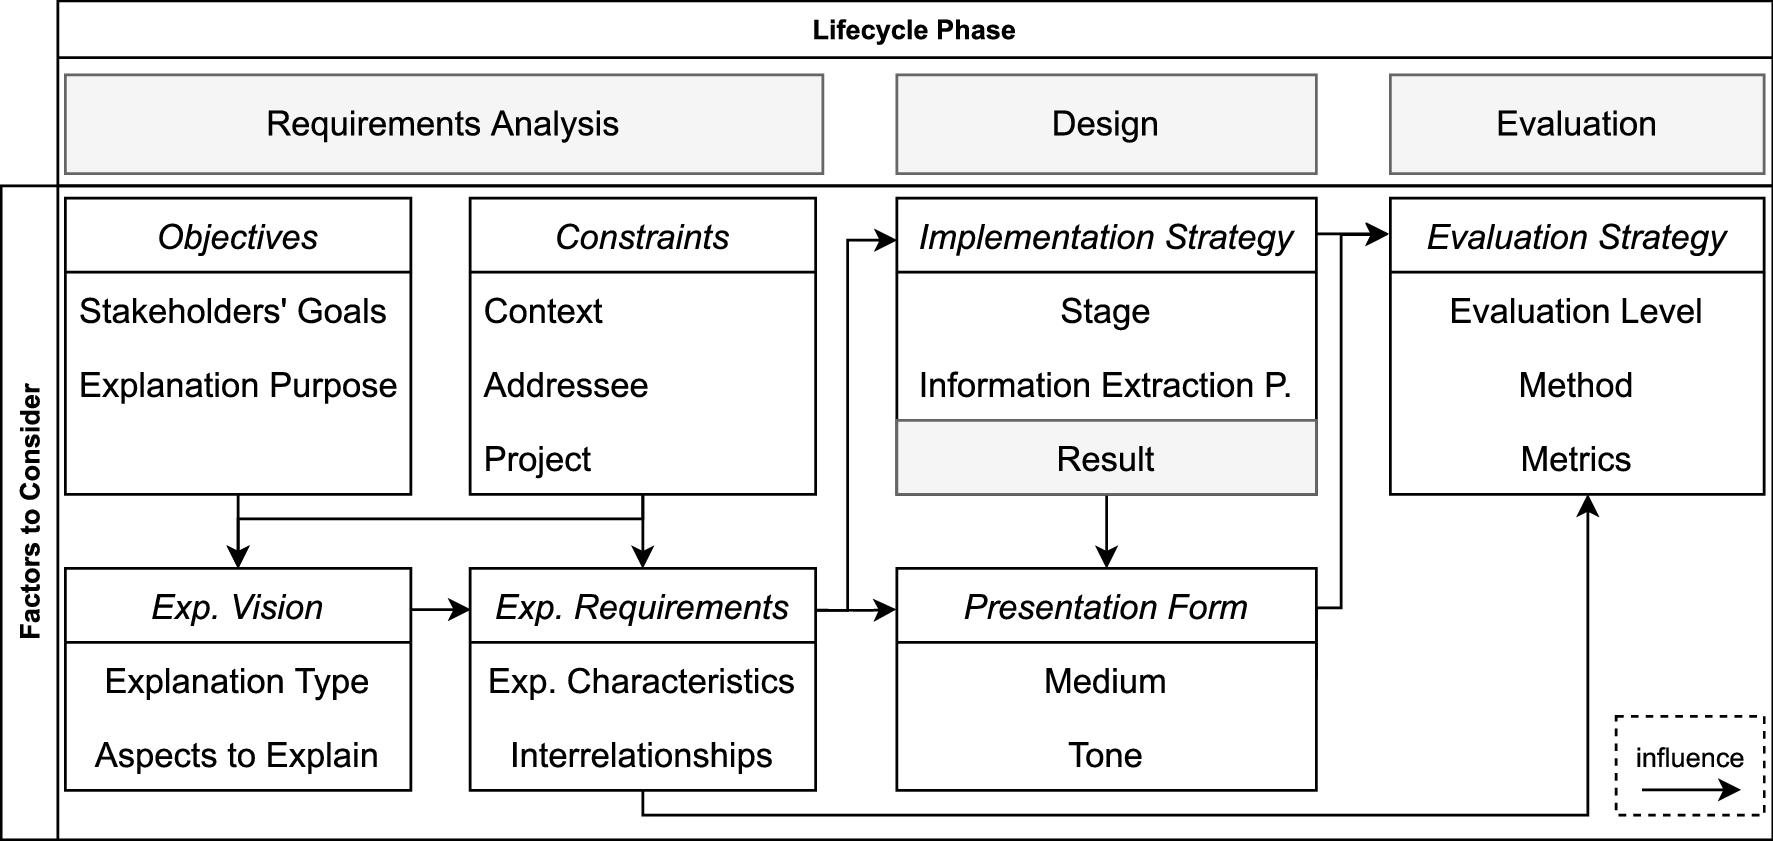
\includegraphics[width=0.9\textwidth]{images/reference_model.png}
    \caption{مدل مرجع برای پشتیبانی از توسعه سیستم‌های توضیح‌پذیر}
    \label{fig:referenceModel}
\end{figure}

مهم‌ترین دلیل استفاده از مدل‌های مرجع را در زیر به دو شکل بیان کرده‌ایم:

\begin{enumerate}
    \item یک چهارچوب یا نمونه‌ای با سطح بالای تجرید، جهت درک کامل روابط میان
    موجودیت‌ها در یک محیط یا دامنه است (مانند شبکه‌های کامپیوتری یا سیستم‌های
    تبیین پذیر)
    \item جهت استانداردسازی یا توصیف فرایند‌های توسعه. ذات این نوع سطح از تجرید
    به مهندسان انعطاف‌پذیری را اعطا می‌کند که می‌توانند در موقعیت‌های مختلف به
    راحتی سازگار شوند.
\end{enumerate}

\begin{figure}[H]
    \centering
    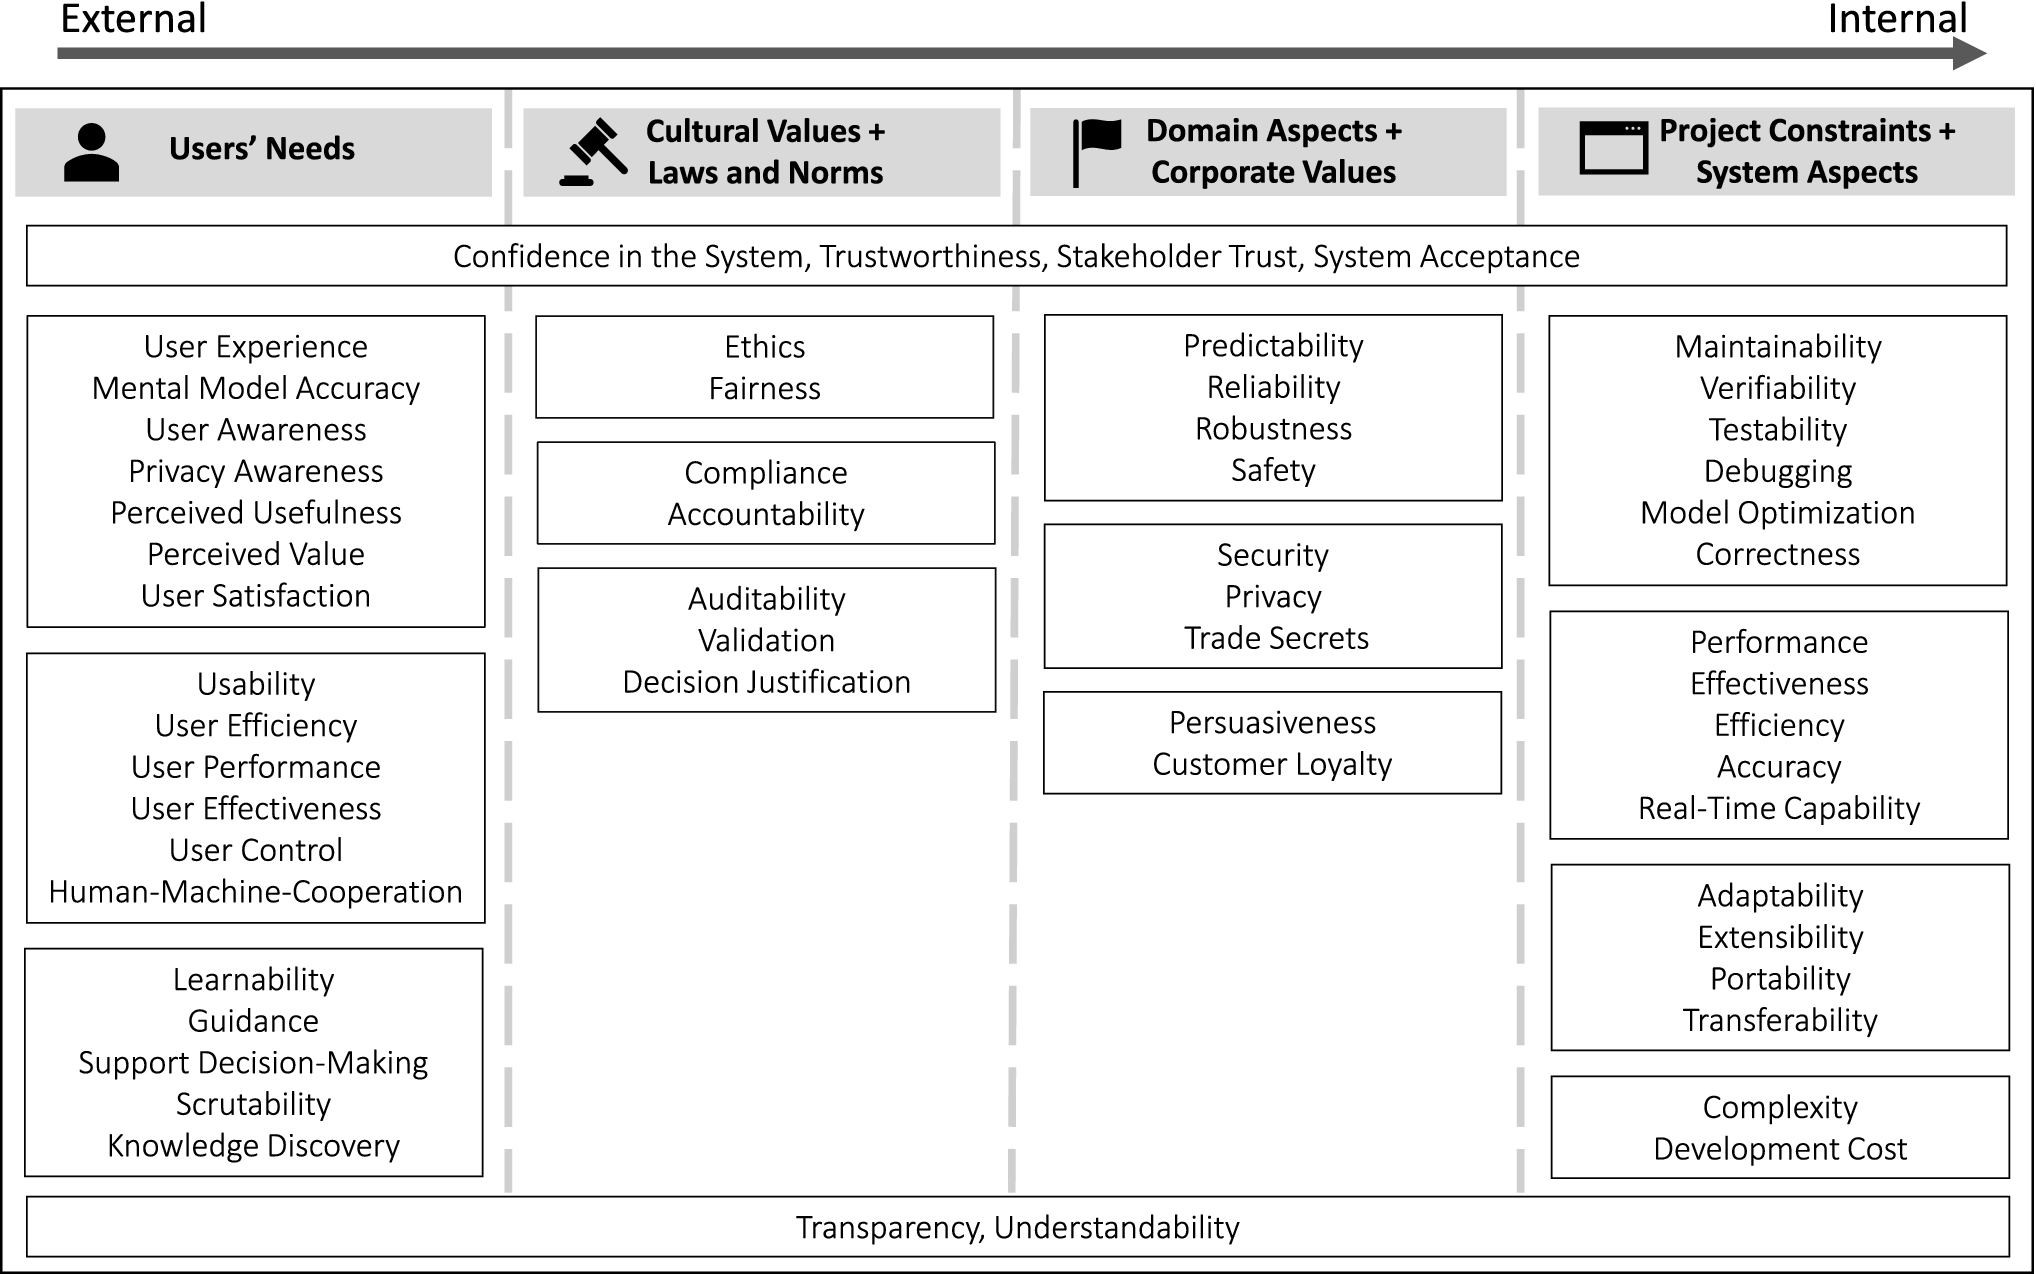
\includegraphics[width=0.9\textwidth]{images/conceptual_model.png}
    \caption{مدل مفهومی که تاثیر توضیح‌پذیری را در ابعاد کیفی مختلف نشان
    می‌دهد.}
    \label{fig:conceptualmodel}
\end{figure}

\subsection{راهنمای شناختی یا \lr{Catalogues}}

کاتالوگ دانش مجموعه‌ای سازمان‌دهی شده از منابع دانشی است که درون یک سازمان وجود
دارد. این منابع می‌توانند شامل انواع دانش‌ها مانند اسناد، گزارش‌ها، روش‌های
توسعه و بهترین رویکرد‌های حل مسئله، مواد آموزشی و موارد دیگر باشند. هدف اصلی از
کاتالوگ‌ها تسهیل در توسعه، به اشتراک‌گذاری و استفاده مجدد از منابع دانش در یک
سازمان در پروژه‌های مشابه می‌باشد. بعضی از محققان کاتالوگی را برای دامنه مشخصی
مبتنی بر فرضیه چهارچوب‌های \lr{NFR} توسعه داده‌اند به گونه‌ای که نتیجه این توسعه
می‌تواند به تریدآف "چگونه یک یا چند \lr{NFR} در یک سیستم رابطه و تعامل دارند و
چگونه می‌توانند با یکدیگر همزستی داشته باشند" بپردازد. از نمونه‌های این
کاتالوگ‌ها می‌توان به موارد زیر اشاره کرد:

\begin{itemize}
    \item \lr{Serrano and Serrano} یک کاتالوگ به طور خاص برای دامنه محاسباتی
    فراگیر و سیار ایجاد کرده‌اند \cite{serrano2013ubiquitous}.
    \item \lr{Torres and Martins} پیشنهاد استفاده از کاتالوگ‌های \lr{NFR} را در
    ساخت برنامه‌های میان‌افزاری \lr{RFID} برای کاهش چالش‌های استخراج داده
    \lr{NFR} در سیستم‌های مستقل، را مطرح کرده‌اند \cite{torres2014nfr}.
\end{itemize}

تمام این نمونه‌ها سعی در این داشتند که کاتالوگ‌ها ابزاری برای کاهش و حذف خطا‌های
احتمالی در شناسایی \lr{FR}ها و \lr{NFR}ها باشند.

\newpage

\section{بررسی رسالت مقاله}

به طور کلی این مقاله از مرور ادبیات سیستماتیک \footnote{\lr{Systematic
Literature Review (SLR)}} استفاده کرده‌است. تعریف توضیح‌پذیری که از این قسمت به
دست می‌آید، نقطه شروع ایجاد یک مدل مهندسی است که تأثیر توضیح‌پذیری را در کنار
سایر ابعاد کیفیت نشان می‌دهد که مورد پذیرش و درک مشترک باشد. سپس فرآورده‌های
مختلفی همچون راهنمای شناختی، مدل مفهومی و مدل مرجع را بر اساس این هسته مفهومی
استخراج و تدوین می‌کند:

\subsection{سوال‌های‌ پژوهشی}

\begin{itemize}
    \item \lr{RQ1}: تعریف مناسب از توضیح‌پذیری برای رسیدن به فهم مشترک در مهندسی
    نیازمندی‌ها و مهندسی نرم‌افزار چیست؟
    \item \lr{RQ2}: حوزه‌های متاثر از توضیح‌پذیری در پس‌زمینه سیستمی چیست؟ چه
    حوزه های کیفی با توجه به زمینه سیستم (دنیای مسأله) از توضیح‌پذیری متاثر
    می‌شود؟
    \item \lr{RQ3}: چگونه توضیح‌پذیری بر سایر حوزه‌های کیفی تاثیر می‌گذارد؟
    \item \lr{RQ4}: چگونه می‌توان به متخصصان نرم‌افزار کمک کرد تا بتوانند
    فاکتورهای حائز اهمیت را در تحلیل، عملیاتی کردن و ارزیابی نیازمندی‌ها برای
    سیستم‌های توضیح‌پذیر مشخص کرد.
\end{itemize}

\subsection*{راه‌حل}

راه‌حل اصلی مرور ادبیات سیستماتیک است. برای ارزیابی و تکمیل یافته‌ها، از یک روش
کیفی دیگر نیز استفاده شده است: دو کارگاه با متخصصان برگزار شد. 

\subsection{استراتژی جست و جو در \lr{SLR}}

\subsubsection{جست و جوی دستی}

در این پژوهش 229 مقاله ۳۶ سال اخیر مورد بررسی قرار گرفته است. این مقالات بین
رشته‌ای و مرتبط با مهندسی نیازمندی‌ها می‌باشند. مقدار $87.0 = k$  نشان‌دهنده
توافق کامل، روی این مقالات بر اساس جست و جو انجام شده می‌باشد. از \lr{open
coding} برای آنالیز داده‌ها جهت تعریف توضیح‌پذیری و رابطه آن با سایر جنبه‌های
کیفی، استفاده کرده است.

\subsubsection{جست و جوی گلوله برفی برای تجمیع و تکمیل نتایج جست و جو}

گردآوری نتایج به صورت پیش رونده و پس رونده بود. این روش بر اساس تئوری \lr{GT}
\footnote{\lr{Grounded Theory}} است. یک مرور ادبیات هیچگاه کامل نمی شود، بلکه به
اشباع می رسد. این اشباع زمانی اتفاق می‌افتد که هیچ مفهوم یا دسته بندی جدیدی از
داده ها به دست نیاید. از این اصل برای پایان دادن به روش گلوله برفی استفاده شده
است. یک تکرار بیشتر در مقالات نداشته‌اند. در تکرار دوم به هیچ دیدگاه یا مفهوم
جدیدی نرسیده‌اند.

\begin{figure}[H]
    \centering
    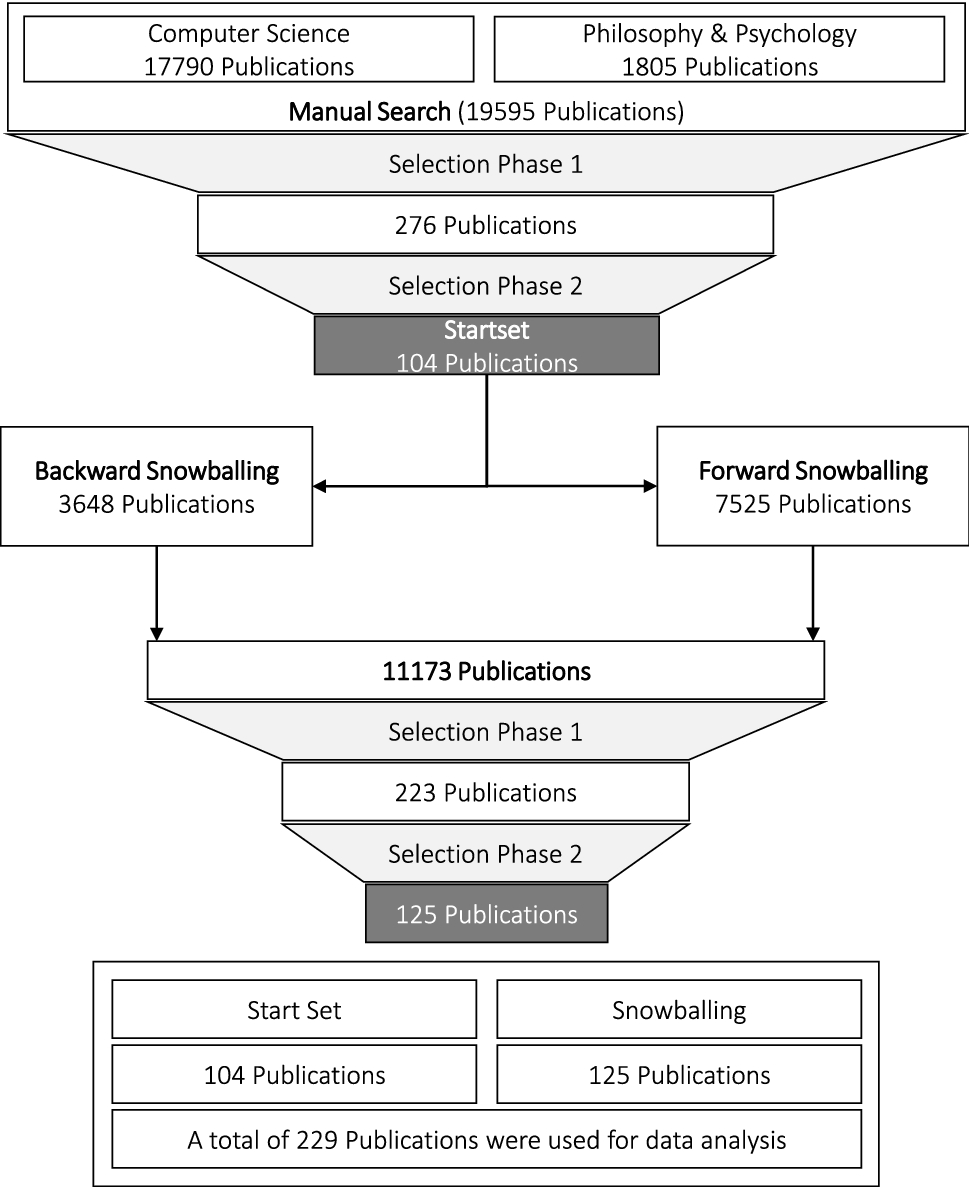
\includegraphics[width=0.5\textwidth]{images/slr_order.png}
    \caption{بررسی ساختار \lr{SLR} انجام شده در این مقاله}
    \label{fig:slrOrder}
\end{figure}

معیارهایی که محققان بر اساس آن‌ها مجموعه‌ای از مقالات را در نظر گرفتند:

\begin{enumerate}
    \item اطلاعاتی که به صورت کامل یا بخشی از سوالات پژوهشی محققان را در بر می‌گرفت.
    \item مقالات در بازه زمانی ژانویه 1984 تا مارس 2020 بوده است. (36 سال) سال
    شروع، اولین باری بوده که کار جدی روی توضیح‌پذیری انجام شده است. سابقه 36
    سال، نشان‌دهنده قدمت و اهمیت موضوع توضیح‌پذیری است.
    \item مقالات شامل پژوهشی، مروری، کنفرانسی و کارگاهی بوده است.
\end{enumerate}

معیارهایی که بر اساس آن ها مقاله‌ها را رد کردند: 

\begin{enumerate}
    \item مقالات غیر انگلیسی زبان
    \item مقالاتی که از تکنیک‌های الگوریتمی استفاده کرده بودند اما درباره
    پس‌زمینه نظری توضیح‌پذیری بحثی نکرده بودند.
\end{enumerate}

انتخاب مقاله یک فرایند دو فازی داشته است:

\begin{enumerate}
    \item انتخاب مقاله بر مبنای عنوان، چکیده و کلمات کلیدی (در این فاز مقالاتی
    که از الگوریتم استفاده می کردند، قابل شناسایی نبودند).
    \item انتخاب مقاله بر مبنای کل متن
\end{enumerate}

اعتبارسنجی داده‌های جمع‌آوری شده با دو کارگاه بوده که در آن متخصصان و خبره‌های
رشته‌های مزبور حضور داشتند. هدف این کارگاه‌ها این بوده که بررسی کنند آیا تمام
داده هایی که نسبت به دامنه جمع آوری شده، درست هستند یا نه؟ نتیجه این بررسی باعث
تولید یک دانشی شده که در قالب مدل مفهومی به صورت شکل در آمده است. این دانش در
ابتدا استخراج شده و سپس تبدیل به اطلاعات ارزشمندی در قالب راهنمای دانش
آماده‌سازی شده است.

\subsection{نتایج: فرآورده‌های پژوهشی}

در مدل مفهومی و کاتالوگ دانش، ارزیابی ذهنی در دسته‌بندی و طبقه‌بندی جنبه‌های
کیفی به ابعاد مختلف، دخالت داشت:

\subsection{راه‌حل این فرآورده‌ها}

\begin{enumerate}
    \item بررسی داخلی: ریشه‌های این طبقه‌بندی بر مفاهیم معتبر موجود در ادبیات
    قرار داده شده است. این طبقه بندی، با کارشناسان مقایسه و بحث شد. 
    \item بررسی خارجی: کارگاه‌ها با کارشناسان برگزار شد. در این مسیر نیز نتایج
    ادبیات با دانش کارشناسی مقایسه شد.
\end{enumerate}

کدگذاری و دسته‌بندی برای مدل مرجع نیز به صورت ارزیابی ذهنی بوده است. برای کاهش
این تهدید، میزان انحراف پژوهشگر را با انجام تحلیل (کدگذاری و دسته‌بندی) به صورت
مستقل کاهش دادیم. چون هدف از برگزاری کارگاه‌ها اعتبارسنجی یافته‌ها نبود، از
نتایج بر پایه کارهای قبلی برای دسته بندی مدل مرجع استفاده شد. با این حال، درستی
و واقع‌گرایی مدل مرجع ارزیابی نشده و نیاز به بررسی‌های بیشتری برای اعتبارسنجی
این مدل وجود دارد.

\subsection{جنبه‌هایی که در این طرح باید توضیح داده شوند}

\begin{itemize}
    \item عملکرد سیستم به طور کلی
    \item فرآیند‌های استدلال سیستم
    \item منطق درونی سیستم
    \item درونی بودن مدل سیستم
    \item قصد و مفهوم سیستم (نتیجه و عملکرد مورد انتظار)
    \item رفتار سیستم و تعامل آن با جهان خارجی
    \item تصمیم‌ها و معیار‌هایی که در تعیین راهبرد‌ها و عملکرد سیستم مورد
    استفاده قرار گرفته است.
    \item شاخص‌های اندازه‌گیری و ارزیابی عملکرد سیستم
    \item دانش سیستم درباره کاربران و جهان خارجی (مطالعه ترجیحات کاربران، دانش
    سیستم درباره جهان و عوامل محیطی مرتبط).
\end{itemize}

\subsection{نتیجه راهنمای شناختی (دانشی)}

در این راهنما دانشی، تأثیر توضیح‌پذیری از دید متخصصان (شرکت‌کنندگان در
کارگاه‌ها) و نیز با توجه به مقاله‌های مورد بررسی (روش \lr{SLR}) بر 57 نیازمندی
غیر عملیاتی، به شرح جدول، فهرست شده است. 

\begin{figure}[H]
    \centering
    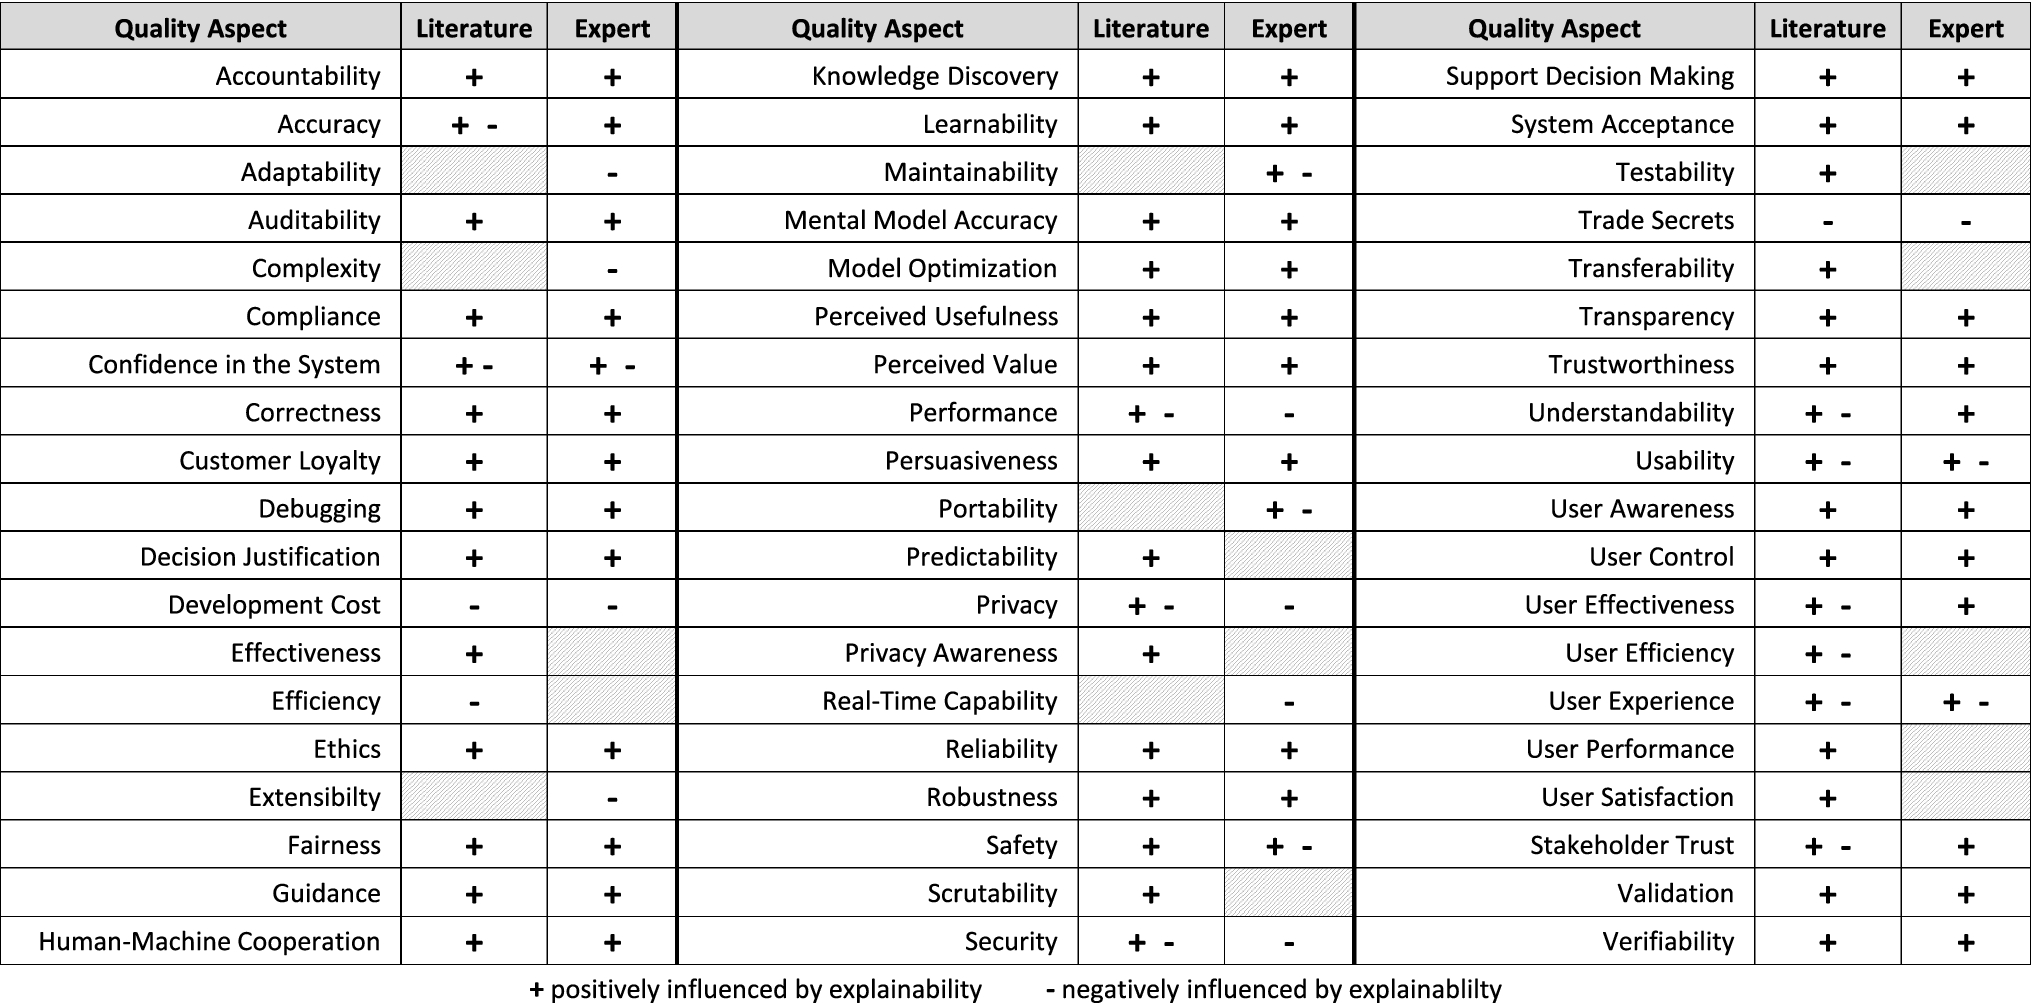
\includegraphics[width=0.9\textwidth]{images/knowledge_catalogue.png}
    \caption{راهنمای دانشی در جهت توضیح‌پذیری و تاثیر آن در جنبه‌های کیفی دیگر}
    \label{fig:resultOfKnowledgeCatalogue}
\end{figure}

\subsection{تجزیه و تحلیل نیازمندی‌ها}

تجزیه و تحلیل نیازمندی‌های جمع آوری شده به منظور درک و مستندسازی آن‌ها می‌باشد.
مواردی که باید درباره آن ها اطلاعات جمع‌آوری و تحلیل کرد، عبارت است از: زمینه
استفاده، جنبه‌های سیستم توضیح‌پذیر و مصرف‌کننده توضیح (سیستم نهایی) .ابعاد کیفی
دیگر به دو صورت روی چگونگی شناسایی توضیح پذیری در سیستم شناسایی، تاثیر دارند؛  

\begin{enumerate}
    \item چه اهدافی با توضیح‌پذیری مشارکت دارند؟ \footnote{مانند شفافیت بیشتر یا
    قابلیت استفاده در یک سیستم}.
    \item محدودیت‌هایی که در سیستم مزبور وجود دارد \footnote{مانند زمان‌بندی
    پروژه یا محدودیت‌های مالی}.
\end{enumerate}

اهداف و محدودیت‌ها به‌عنوان پایه‌ای برای تصمیمات سطح بالاتر، مانند تعریف یک
دیدگاه توضیح‌پذیری، عمل می‌کنند. دیدگاه توضیح‌پذیری تعریفی سطح بالا از
توضیح‌پذیری است و شامل ملاحظاتی مانند نوع توضیحی که ارائه می‌شود و جنبه‌های مهم
برای توضیح است. علاوه بر این، تمام این ملاحظات (اهداف، محدودیت‌ها، دیدگاه
توضیح‌پذیری) در نهایت در نیازمندی های توضیح‌پذیری جمع‌آوری می‌شوند.

\subsection{اهداف}

شامل اهداف نهایی ذینفعان و دلایل نیاز به توضیح‌پذیری در یک سیستم است. این
خواسته‌ها، دلایل و اهداف، متعاقباً به وسیله هر یک از ابعاد کیفیتی که قبلاً ذکر
شد (مانند ارزش‌های فرهنگی، جنبه‌های دامنه و...) تحت تاثیر قرار می‌گیرند.
توضیح‌پذیری می‌تواند ابزار دستیابی به جنبه‌های دیگر کیفی باشد که باید به آن جنبه
تصریح شود. ممکن است در یک پروژه خاص ذینفعان بخواهند جنبه‌های دیگر کیفیت مانند
بهبود تجربه کاربری یا نیاز به توسعه یک سیستم در هماهنگی با ارزش‌های اخلاقی از
طریق توضیح‌پذیری تحقق یابد. به طور کلی، همه یا هر کدام از ۵۷ جنبه کیفیتی که در
مدل شکل شماره. \ref{fig:resultOfKnowledgeCatalogue} لیست شده‌اند، در هر ترکیبی
می‌توانند به عنوان یک هدف عمل کنند.

\subsection{محدودیت‌ها}

محدودیت‌ها عواملی هستند که به طور مستقیم یا غیرمستقیم تصمیم‌گیری‌های طراحی را
تحت تأثیر قرار می‌دهند یا محدود می‌کنند. محدودیت‌ها با عواملی مانند زمینه
\footnote{زمینه، تعامل فرد (برای مثال پزشک)، سیستم (سیستم تشخیص سرطان
توضیح‌پذیر)، وظیفه (پشتیبانی از تفسیر آزمایش‌های تصویری تومور‌های سرطانی) و محیط
(بیمارستان) است.} گیرنده و شرایط پروژه مرتبط هستند. این عوامل تاثیر قابل توجهی
بر طراحی سیستم می گذارند. همه این تأثیرات باید در نظر گرفته شوند تا یک دیدگاه از
سیستمی که قرار است توسعه یابد تعریف شود و آن را به نیازمندی‌ها تبدیل کند.
محدودیت‌ها باعث اعمال و شکل گرفتن تصمیمات طراحی خاص می‌شوند.

\subsection{استراتژی پیاده‌سازی}

استراتژی پیاده‌سازی به این معنا است که چگونه توضیحات در سیستم پیاده‌سازی
می‌شود. این بخش شامل توابع، ماژول‌ها (از نظر راه‌حل‌های الگوریتمی) و عناصر رابط
کاربری است که باید در سیستم پیاده‌سازی شود تا توضیحات ارائه شود.

\begin{itemize}
    \item توابع می‌توانند بسته به آنچه باید توضیح داده شود و پیچیدگی مدل
    زیربنایی، از نظر پیچیدگی متفاوت باشند.
    \item ماژول‌ها به عنوان بخش مجزا از سیستم و یک موجودیت جداگانه عمل می‌کنند.
    (به عنوان مثال، یک دستیار مجازی). 
    \item در نهایت، عوامل رابط کاربری بیشتر مربوط به انتخاب‌های طراحی مربوط به
    این است که توضیحات چگونه در رابط کاربری ارائه خواهد شد.
\end{itemize}

\subsection{بررسی و دو مرحله برای پیاده‌سازی توضیح‌پذیری}

سیستم‌های توضیح‌پذیر را می‌توان در دو مرحله بررسی کرد:

\begin{enumerate}
    \item مرحله پسازمان: توضیح سیستم فعلی، پس از طراحی و پیاده‌سازی
    \item مرحله پیش از زمان: قبل از طراحی و پیاده‌سازی سیستم، توضیح‌پذیری را در
    آن و نیازمندی‌های آن اعمال می‌کنیم و سپس سیستم مورد نظر را توسعه می‌دهیم.
\end{enumerate}

\section{روال استخراج اطلاعات برای ایجاد توضیحات}
این که چگونه اطلاعات مورد نیاز برای ایجاد توضیحات استخراج می‌شود. استخراج
اطلاعات برای سیستم‌های مبتنی بر هوش مصنوعی اغلب باید توسط یک ماژول اضافی انجام
می شود.

در سیستم های سنتی این سوال مطرح است که آیا دسترسی به کد سیستم برای به دست آوردن
اطلاعات مورد نیاز برای توضیح آن ضروری است؟ با دسترسی کد می توان آن را تحلیل
کرده، به الگوریتم رسید و اطلاعات داخلی را که برای ساخت توضیحات استفاده می‌شود،
به دست آورد.  در واقعیت، دسترسی به کد سیستم ضروری نیست، چون می‌توان اطلاعات مورد
نیاز برای ایجاد توضیحات را از طریق تجزیه و تحلیل‌های خارجی جمع‌آوری کرد. برای
این کار می توان از روش اختلال محلی استفاده کرد. در این روش، ورودی را دست کاری می
کنیم تا چگونگی تغییرات خروجی را ببینیم.

\subsection{نتیجه استخراج اطلاعات}

اطلاعات استخراج شده، معمولاً دارای یک معنای خاص است که به آن نتیجه می‌گویند.
انتخاب دقیق معنای یک توضیح ممکن است حیاتی باشد، به توجه به اینکه چه کسی توضیح را
دریافت می‌کند و در چه زمینه‌ای تولید می‌شود. این اتفاق ممکن است رخ دهد زیرا
معنای یک توضیح معمولاً کسانی را که می‌توانند آن را درک کنند، تحت تأثیر قرار
می‌دهد.

انواع مختلف نتایج:

\begin{enumerate}
    \item وابستگیِ ویژگی: اطلاعات استخراج شده می‌تواند به وابستگی ورودی و خروجی
    در یک ویژگی اشاره کند. 
    \item مثال‌ها: ممکن است مثال‌های نماینده از تصمیمات مشابه باشند.
    \item پیوندهای به توضیح: به عنوان مثال، روشن کردن یک ویژگی خاص می‌تواند برای
    پیاده‌سازی توضیحات متضاد استفاده شود و توضیحات علیتی می‌توانند با ارائه
    مثال‌ها منتقل شوند.
\end{enumerate}

\subsection{فرم ارائه}

توضیحات می‌توانند به صورت‌های مختلف متنی، عددی، تصویری و شنیداری باشند. هرکدام
از این فرمت‌ها دارای زیر-کلاس‌های دیگری است. به عنوان مثال، فرمت‌های متنی
می‌توانند به زبان طبیعی و یا به صورت قوانین (مثلاً دستورات \lr{if-else}) باشند. 
توضیحات باید با استراتژی‌های طراحی خاص رابط کاربری مانند توضیحات شنیداری،
آیکون‌ها و انیمیشن‌ها (مثلاً برای برجسته کردن رویدادی جدید مانند یک رخداد) در
صفحه‌نمایش کامپیوتر باشند و به طور احتمالی با متن‌های مختصر ارائه شوند. علاوه بر
این، لحن ارتباطی باید غیررسمی باشد و نه رسمی.

\subsection{استفاده از ماژول توضیحات}

می‌توان برای ارائه توضیحات در سیستم‌های مبتنی بر هوش مصنوعی، یک ماژول به سیستم
موجود اضافه کرد. این روش از نظر مرحله پسا زمان خواهد بود. وقتی می توان از ماژول
توضیحات استفاده کرد که سیستم مورد نظر، به وسیله شبکه عصبی عمیق (\lr{DNN})
پشتیبانی ‌شود. بنابراین، روش استخراج اطلاعات ماژول باید با \lr{DNN} ها سازگار
باشد

\section{ارزیابی}

ارتباطات پلی بین اهداف کلی مشتری به یک سو و معیارهای موافقت‌ شده برای
اندازه‌گیری به سوی دیگر می‌سازند. به همین ترتیب، برای تحلیل تأثیر توضیحات،
روش‌ها و معیارهای ارزیابی باید تعریف شوند. به طور خاص، معیارها باید کمک کنند تا
متوجه شویم آیا راه‌حل‌های فنی انتخابی به تأمین نیازمندی‌های تعریف‌شده کمک
می‌کنند؟ همچنین به ارزیابی نیز کمک می‌کنند؟ آیا اجرای انتخاب‌ شده برای قابلیت
توضیح مناسب است؟ یا نیاز به بهبود دارد؟

\subsection{سطوح ارزیابی برای توضیح‌پذیری}

حداقل دو سطح ارزیابی برای توضیح‌پذیری می‌توان در نظر گرفت:

\subsubsection{ارزیابی در سطح سیستم}

توضیح‌پذیری جنبه فعال‌سازی دارد و با آن می‌توان به \lr{NFR}های دیگر دست پیدا
کرد. پس می‌توانیم توضیح‌پذیری را با اندازه‌گیری میزان مشارکت آن در دست‌یابی به
جنبه‌های کیفیت دیگر ارزیابی کنیم. مثلا می‌توان از مشارکت توضیح‌پذیری و استفاده
پذیری \footnote{ به عنوان مثال کلمه \lr{Usability} تأثیر توضیحات بر
استفاده‌پذیری سیستم می‌تواند به‌صورت کمی (از طریق نمرات آزمون‌های استفاده‌پذیری)
یا به‌صورت کیفی (از طریق ارزیابی درک کاربران از استفاده‌پذیری سیستم) ارزیابی
شود.} و یا عملکرد، به ارزیابی آن پرداخت.

\subsubsection{ارزیابی در سطح توضیح}

می‌توانیم توضیح‌پذیری را با وارسی توضیحات تولید شده نیز ارزیابی کنیم. روش‌های
مختلف برای ارزیابی توضیحات سیستم‌های نرم‌افزاری در سطح توضیح پیشنهاد شده است. با
این حال، این روش‌ها استانداردی ندارد و انتخاب روش‌های ارزیابی و معیارهای آن به
اهداف از پیش تعیین شده، وابسته است.

\subsection{روش‌های ارزیابی}

محققان در این مقاله روش‌هایی را برای ارزیابی شناسایی کرده‌اند عبارتند از:

\begin{itemize}
    \item مطالعات کاربری به طور کلی
    \item پرسشنامه‌ها
    \item آزمون‌های \lr{A/B}
    \item مطالعات موردی
    \item مصاحبه‌ها
\end{itemize}

\subsection{بررسی بازخورد کاربران نهایی}

بررسی بازخوردهای کاربران نهایی: مهم‌ترین روش‌های استفاده شده برای ارزیابی
توضیحات، مطالعات کاربری هستند. ارزیابی‌های ذهنی، روش متداول‌تری برای ارزیابی
هستند. فعالیت‌ها و روش‌های متمرکز بر روی کاربر، اغلب برای توسعه سیستم‌های توضیح
پذیر توصیه می‌شوند. در این تحقیق، محققان در SLR خود یافته‌اند که مهم‌ترین
روش‌های ارزیابی بر روی بازخوردهای کاربران نهایی تمرکز دارد.

\subsection{پرسشنامه}

در پرسشنامه‌ها، شرکت‌کنندگان مطالعه ممکن است سوال شوند که آیا یک جنبه خاص از
سیستم را پس از دریافت توضیحات بهتر درک کرده‌اند یا خیر. به عنوان مثال: "از
توضیحات، من نحوه عملکرد [نرم‌افزار، الگوریتم، ابزار] را می‌فهمم."

\subsection{آزمون‌های \lr{A/B}}

در این روش، دو یا چند نسخه یا نوع مختلف از یک عنصر (مثلاً توضیحات) به صورت
تصادفی به گروه‌های مختلف از کاربران ارائه می‌شود. یک گروه (گروه \lr{A}) نسخه
اصلی یا قدیمی را دریافت می‌کند و دیگر گروه (گروه \lr{B}) نسخه جدید یا تغییر
یافته را دریافت می‌کند. سپس به هر گروه پرسیده می‌شود که کدام نسخه را ترجیح
می‌دهند یا چگونگی تاثیر آن را ارزیابی می‌کنند. این روش به تحلیل تاثیر تغییرات و
انجام مقایسه بین دو یا چند شرایط یا نسخه مختلف برای انتخاب بهترین گزینه برای
مدیریت و بهبود سیستم کمک می‌کند.

\subsection{مطالعات موردی}

یک روش تحقیق تجربی که بر روی مطالعه یک مورد یا پدیده خاص (مانند یک فرد، یک گروه،
یک محیط، یا یک سازمان) در محیط یا متن خود تمرکز دارد. در مطالعات موردی از ترکیب
چندین تکنیک جمع‌آوری داده استفاده می‌کنند تا به درک بهتر پیچیدگی موارد فردی کمک
کند و دقت داده‌ها و استنتاج‌های حاصل را افزایش‌دهد. یک مطالعه موردی ممکن است
شامل ارزیابی سیستم‌های توضیح‌پذیر در یک محیط خاص و استخراج اطلاعات دقیق در مورد
تأثیر آنها باشد.

\subsection{مصاحبه}

یک روش تحقیق کیفی است که در آن جمعیت مورد نظر (یعنی افرادی که مورد مصاحبه قرار
می‌گیرند) توسط پژوهشگر پرسش می‌شوند.

\section{معیارها}

ابزارهای سنجش متنوعی برای توضیح‌پذیری وجود دارد. سازگاری، پذیرفته‌شدن،
واقع‌گرایی و متقاعدسازی می‌توانند برای سنجش توضیحات به کار روند. قابلیت فهم،
ارتباط، طول، به‌موقع بودن، کامل بودن، و سودمندی نیز از معیارهایی است که در پژوهش
های پیشین بسیار مطرح شده است. به‌موقع بودن توضیح، یک محدودیت است. یک توضیح وقتی
کمک‌کننده یا مرتبط است که نه تنها جامع باشد، بلکه در لحظه‌ مناسب بیان شود تا در
تصمیم‌گیری کمک کند. مثلا در هنگام مسیریابی، توضیحی که دلایل تغییر مسیر را شرح
می‌دهد باید به موقع فهمیده شود تا مسافر بتواند به موقع تصمیم بگیرد. در این
سناریو، حد فاصل زمانی که کاربر توضیحات را دریافت می‌کند تا زمان انجام اقدام،
می‌تواند یک معیار در نظر گرفته شود. مثلا این معیار می‌تواند برای ارزیابی این
استفاده شود که آیا کاربر توضیح تغییر مسیر را در زمان مناسب به دست آورده یا آیا
هنوز فاصله‌هایی در انتقال اطلاعات وجود دارد. سرانجام، یک مطالعه کاربری می‌تواند
به ارزیابی نگرش شرکت‌کنندگان نسبت به تجربه کاربری کمک کند. 

\section{کلیات و مباحث}

اولین کاری که در این پژوهش مورد بررسی قرار گرفت، تعریف توضیح‌پذیری برای مهندسان
نرم‌افزار است. این تعریف مشخص می‌کند هنگام مدیریت نیازمندی‌ها و عملکرد مناسب
برای سیستم‌های توضیح‌پذیر چه چیزی باید در نظر گرفته شود:

\begin{itemize}
    \item جنبه‌هایی که باید توضیح داده شوند.
    \item زمینه‌ها، توضیح‌دهندگان و مخاطبان 
\end{itemize}

علاوه‌بر این، آگاهی از این متغیرها فرآیند توسعه نرم‌افزار را تسهیل و حمایت
می‌کند و نیازمندی‌های توضیح‌پذیری را مشخص می‌کند.  از آن جا که توضیح‌پذیری به
عنوان یک جنبه ارتباطی بین سیستم‌ها و انسان‌ها دیده می شود، بسته به اینکه چگونه
در عمل اتفاق می‌افتد، می‌تواند روابط را تقویت یا آن‌ها را آسیب بزند.از طرف دیگر،
انتخاب‌های طراحی نادرست در خصوص توضیح‌پذیری می‌تواند مشکلات زیر را به وجود آورد:

\begin{enumerate}
    \item ارائه‌ی اطلاعات ناکافی یا انتخاب‌ ارائه‌ نادرست: بر روابط با کاربر
    مثلاً مشکلات تجربه‌ کاربری تاثیرات منفی بگذارد.
    \item تاثیر نابجا در جنبه‌های کیفی ضروری برای شرکت ها: مثلاً برای تصویر برند
    و وفاداری مشتری آسیب جدی داشته باشد.
    \item ایجاد تاثیرات منفی برای پروژه یا سیستم: مثلاً هزینه‌های توسعه را
    افزایش دهد یا موجودیت سیستم را مختل کند.
\end{enumerate}

\subsection{محدودیت‌ها و تهدید اعتبار پژوهش}

اساس این پژوهش، تحلیل داده‌های کیفی است. بنابراین، احتمال وابستگی نتایج به زمان
تحلیل و احتمال وجود اختلافات زیادی در نتایج وجود دارد. بنابراین، از یک رویکرد
چند روشی استفاده شده تا نتایج ارائه شده از جامعیت و اعتبار بالاتری برخور باشند.
این روش ها عبارتند از:

\subsubsection{انجام یک مرور سیستماتیک و فرآیند کدگذاری}

در این قسمت معیار‌هایی وجود دارد که می‌تواند پیش از شروع مرور ادبیات، برای رسیدن
به یک سطح مناسب از فهم مشترک تدوین شده باشد تا تمام تهدید‌های اعتبار این پژوهش
را کاهش دهد:

\begin{enumerate}
    \item معیارهای اضافه و کاهش برای جلوگیری از تصمیمات ذهنی موضوعی در فرآیند
    انتخاب.
    \item معیار دوره انتشار، که قابل ارزیابی است.
    \item معیارهای وابسته به محتوای مقالات که به موضوع هستند.
    \item برای کاهش میزان تعصب پژوهشگر، تحلیل به صورت مستقل انجام شد.
    \item در هر دو مرحله بررسی ادبیات و فرآیند کدگذاری، در صورت عدم توافق، تصمیم
    در مورد اضافه یا حذف (برای یک مقاله) یا اختصاص کد (برای داده‌های استخراج
    شده) به صورت جمعی تصمیم گرفته شده است.
\end{enumerate}

یکی از محدودیت‌های دیگر مرور فرآیند پژوهش این است که تنها دوره زمانی تا مارس
۲۰۲۰ را پوشش می‌دهد. توضیح‌پذیری یک زمینه تحقیقاتی به سرعت در حال تکامل است،
تضمینی برای به‌روز بودن نتایج محققان وجود ندارد. برای کاهش این مشکل، هنگام ساخت
مدل مرجع از تحقیقات جدیدتر به عنوان راهنمایی استفاده شده است. در این زمینه، هیچ
مشکلی برای به اجماع رسیدن نتایج محققان وجود نداشته است. علاوه بر این، دوره زمانی
مرور پژوهش در حال حاضر شامل 36 سال است، در طی آن مشاهده کردیم که مفاهیم مشابه
ثابت در ادبیات باقی می‌مانند.

\subsubsection{کارگاه‌ها}

برای کارگاه‌ها چندین تهدید به اعتبار وجود دارد:

\begin{enumerate}
    \item برخی از تکالیف داده شده به شرکت‌کنندگان بر اساس نتایج بررسی ادبیات
    پژوهش بوده است که ممکن است افراد را به طور ضمنی تحت تاثیر قرار دهد. 
    \begin{enumerate}
        \item راه حل: تمام اطلاعات اضافی از تکالیف حذف شد. همچنین، کارشناسان
        می‌توانستند از تجربیات خود استفاده کنند و محدودیتی نداشتند.
    \end{enumerate}
    \item کارگاه‌ها به صورت آنلاین برگزار شد که می‌تواند یک عامل محدود‌ کننده
    باشد. در اینجا، هدف از تکالیف این بوده است که کارشناسان را با موضوع آشنا کند
    تا کارگاه‌ها به طور متمرکز در میان فرمت آنلاین برگزار شوند. 
    \begin{enumerate}
        \item راه حل: از مکث‌های زیاد و وظایف واضح استفاده شد و این کمک کرد تا
        شرکت‌کنندگان در طول کارگاه بهره‌وری داشته باشند.
    \end{enumerate}
    \item زمان اختصاص داده شده برای هر کارگاه کوتاه بود. چهار ساعت برای هر کدام.
    \begin{enumerate}
        \item راه حل: فقط سه وظیفه برای هر کارگاه در نظر گرفته شد. محدود کردن
        کارها باعث شد کارگاهی لغو نشود (اشاره به کتاب کار آهسته کال نیوپورت
        \cite{slowProductivity}).
    \end{enumerate}
\end{enumerate}

\section{نتیجه‌گیری نهایی و ایده‌ها}

توضیح‌پذیری یک وسیله مناسب برای دستیابی به جنبه‌های کیفی ضروری در یک سیستم،
مانند شفافیت، پاسخگویی و اعتماد است. با جانمایی این جنبه ها در سیستم‌ها، به
ابزارها و روش‌هایی برای تحلیل، پیاده‌سازی و اعتبارسنجی نیازمندی های مرتبط احساس
نیاز می‌شود. به همین دلیل، باید موافقت راجع به درک توضیح‌پذیری به طور کلی داشته
باشیم. معنی آن، اثرات آن، دسته‌بندی آن. علاوه بر این، تأثیر توضیح‌پذیری با
جنبه‌های کیفی مهم‌تری مانند اخلاق، حریم خصوصی و اعتماد همچنین باید مورد تحقیق
قرار گیرد.

تعریف توضیح پذیری ارائه شده در این پژوهش، به فرآیند ارتباط و انطباق انتظارات
هنگام اشاره به توضیح‌پذیری کمک می کند. مدل مفهومی به متخصصان کمک می کند تا
دسته‌بندی های توضیح پذیری را درک کنند. کاتالوگ دانش به شناسایی تفاوت ها بین
توضیح‌پذیری و سایر کیفیت‌های مهم کمک می کند. مدل مرجع پیشنهادی برای توضیح‌پذیری
به مهندسین نرم‌افزار کمک می کند تا جنبه‌های مرتبط و تاثیرگذار برای تجزیه و تحلیل
نیاز‌ها، طراحی و ارزیابی سیستم‌های توضیح پذیر را درک کنند. به عنوان پیشنهاد
پژوهش، با پشتیبانی از این آرتیفکت ها، می توان به استراتژی‌های طراحی و راه‌حل‌های
سطح اجرا دست پیدا کرد که به نتایج مثبت برای همه ذینفعان منجر می‌شود. 